\chapter{Implémentations artistiques}

\label{ch:Implémentations aristiques}

\section{\textit{Introduction}}


This section concludes an artistic point of view of the aspects discussed in the previous chapters. Starting from the Fourier transform to the phase vocoder and ending to morphing artistic interpretations of the implemented technical Max patches.

The goal of this chapter is to support the idea that spectral analysis and resynthesis and in expansion musical signal processing is useful both to scientifics and artists. Indeed the previous extensively technical details come to use for artistic and aesthetical purposes. The following examples consist of personal experimentation and interpretation of the technical material already presented.


Cette section conclut un point de vue artistique sur les aspects abordés dans les chapitres précédents. À partir de la transformation de Fourier en vocodeur de phase et en passant au morphing par des interprétations artistiques des patchs techniques mis en œuvre.

L'objectif de ce chapitre est de soutenir l'idée que l'analyse et la re-synthèse spectrales, et donc en expansion, le développement du signal musical  sont utiles aux scientifiques et aux artistes. En effet, les détails techniques antérieurs sont utilisés à des fins artistiques et esthétiques. Les exemples suivants consistent en une expérimentation personnelle et une interprétation du matériel technique déjà présenté.

\section{Le vocodeur de phase - \textit{Une capacité sans fin}}

\subsection{Super Phase Vocoder}

For the purpose of combining mulptiple techniques of the phase vocodeur we implementated a Super Phase Vocoder. This spectral tool includes time streching, time freeze, pitch shifting, morphing and other effects beneficiating from the basic function of the phase vocoder.


Dans le but de combiner plusieurs techniques du vocodeur de phase, nous avons implémenté un \guillemotleft \textit{super} vocodeur de phase\guillemotright . Cet outil spectral comprend l'étirement temporel, le freeze temporel, le décalage de hauteur, le morphing et d'autres effets bénéficiant de la fonction élémentaire du vocodeur de phase.

The graph \ref{FirstMorphingTry} displays the control window of all parameters for the phase vocoder. This version of the phase vocoder contains every effect that was investigated in the previous section. There is not something particularly different from the basic phase vocoder for morphing but some more functionalities. It is only natural to seek for a larger functionality for the same tool. Thus, we implemented every basic effect into a single patch. The math here are not interesting to analyse as they were all seen before. The most crucial details are in the sequencing of all effects that can be visualized in figure \ref{SuperPhaseVoc}.


	\begin{figure}
        \centering
        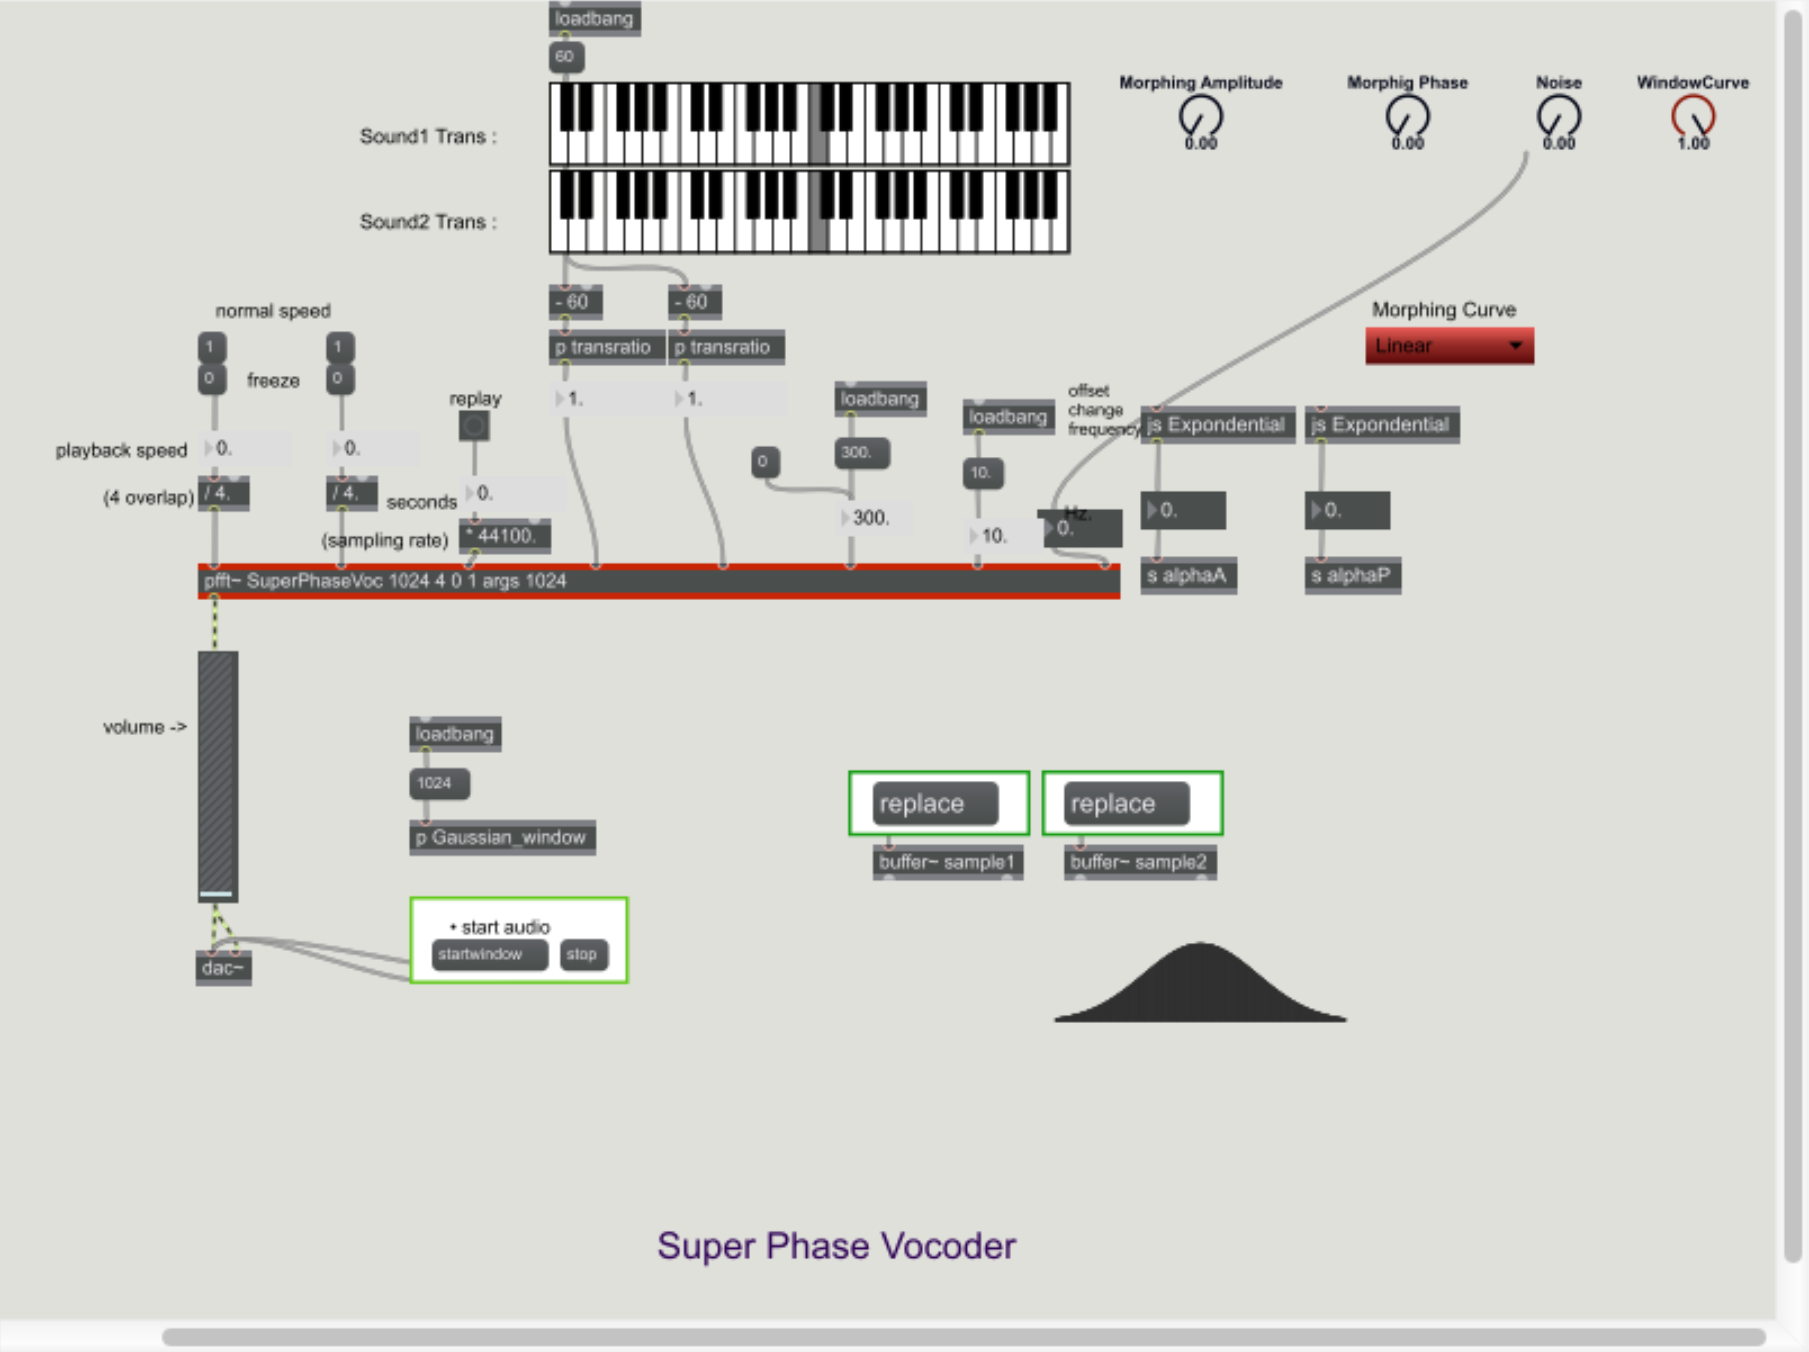
\includegraphics[width = \textwidth]{Graphs/FirstMorphingTry.png}
        \caption{Super Phase Vocoder I}
        \label{FirstMorphingTry}
    \end{figure}



	\begin{figure}
        \centering
        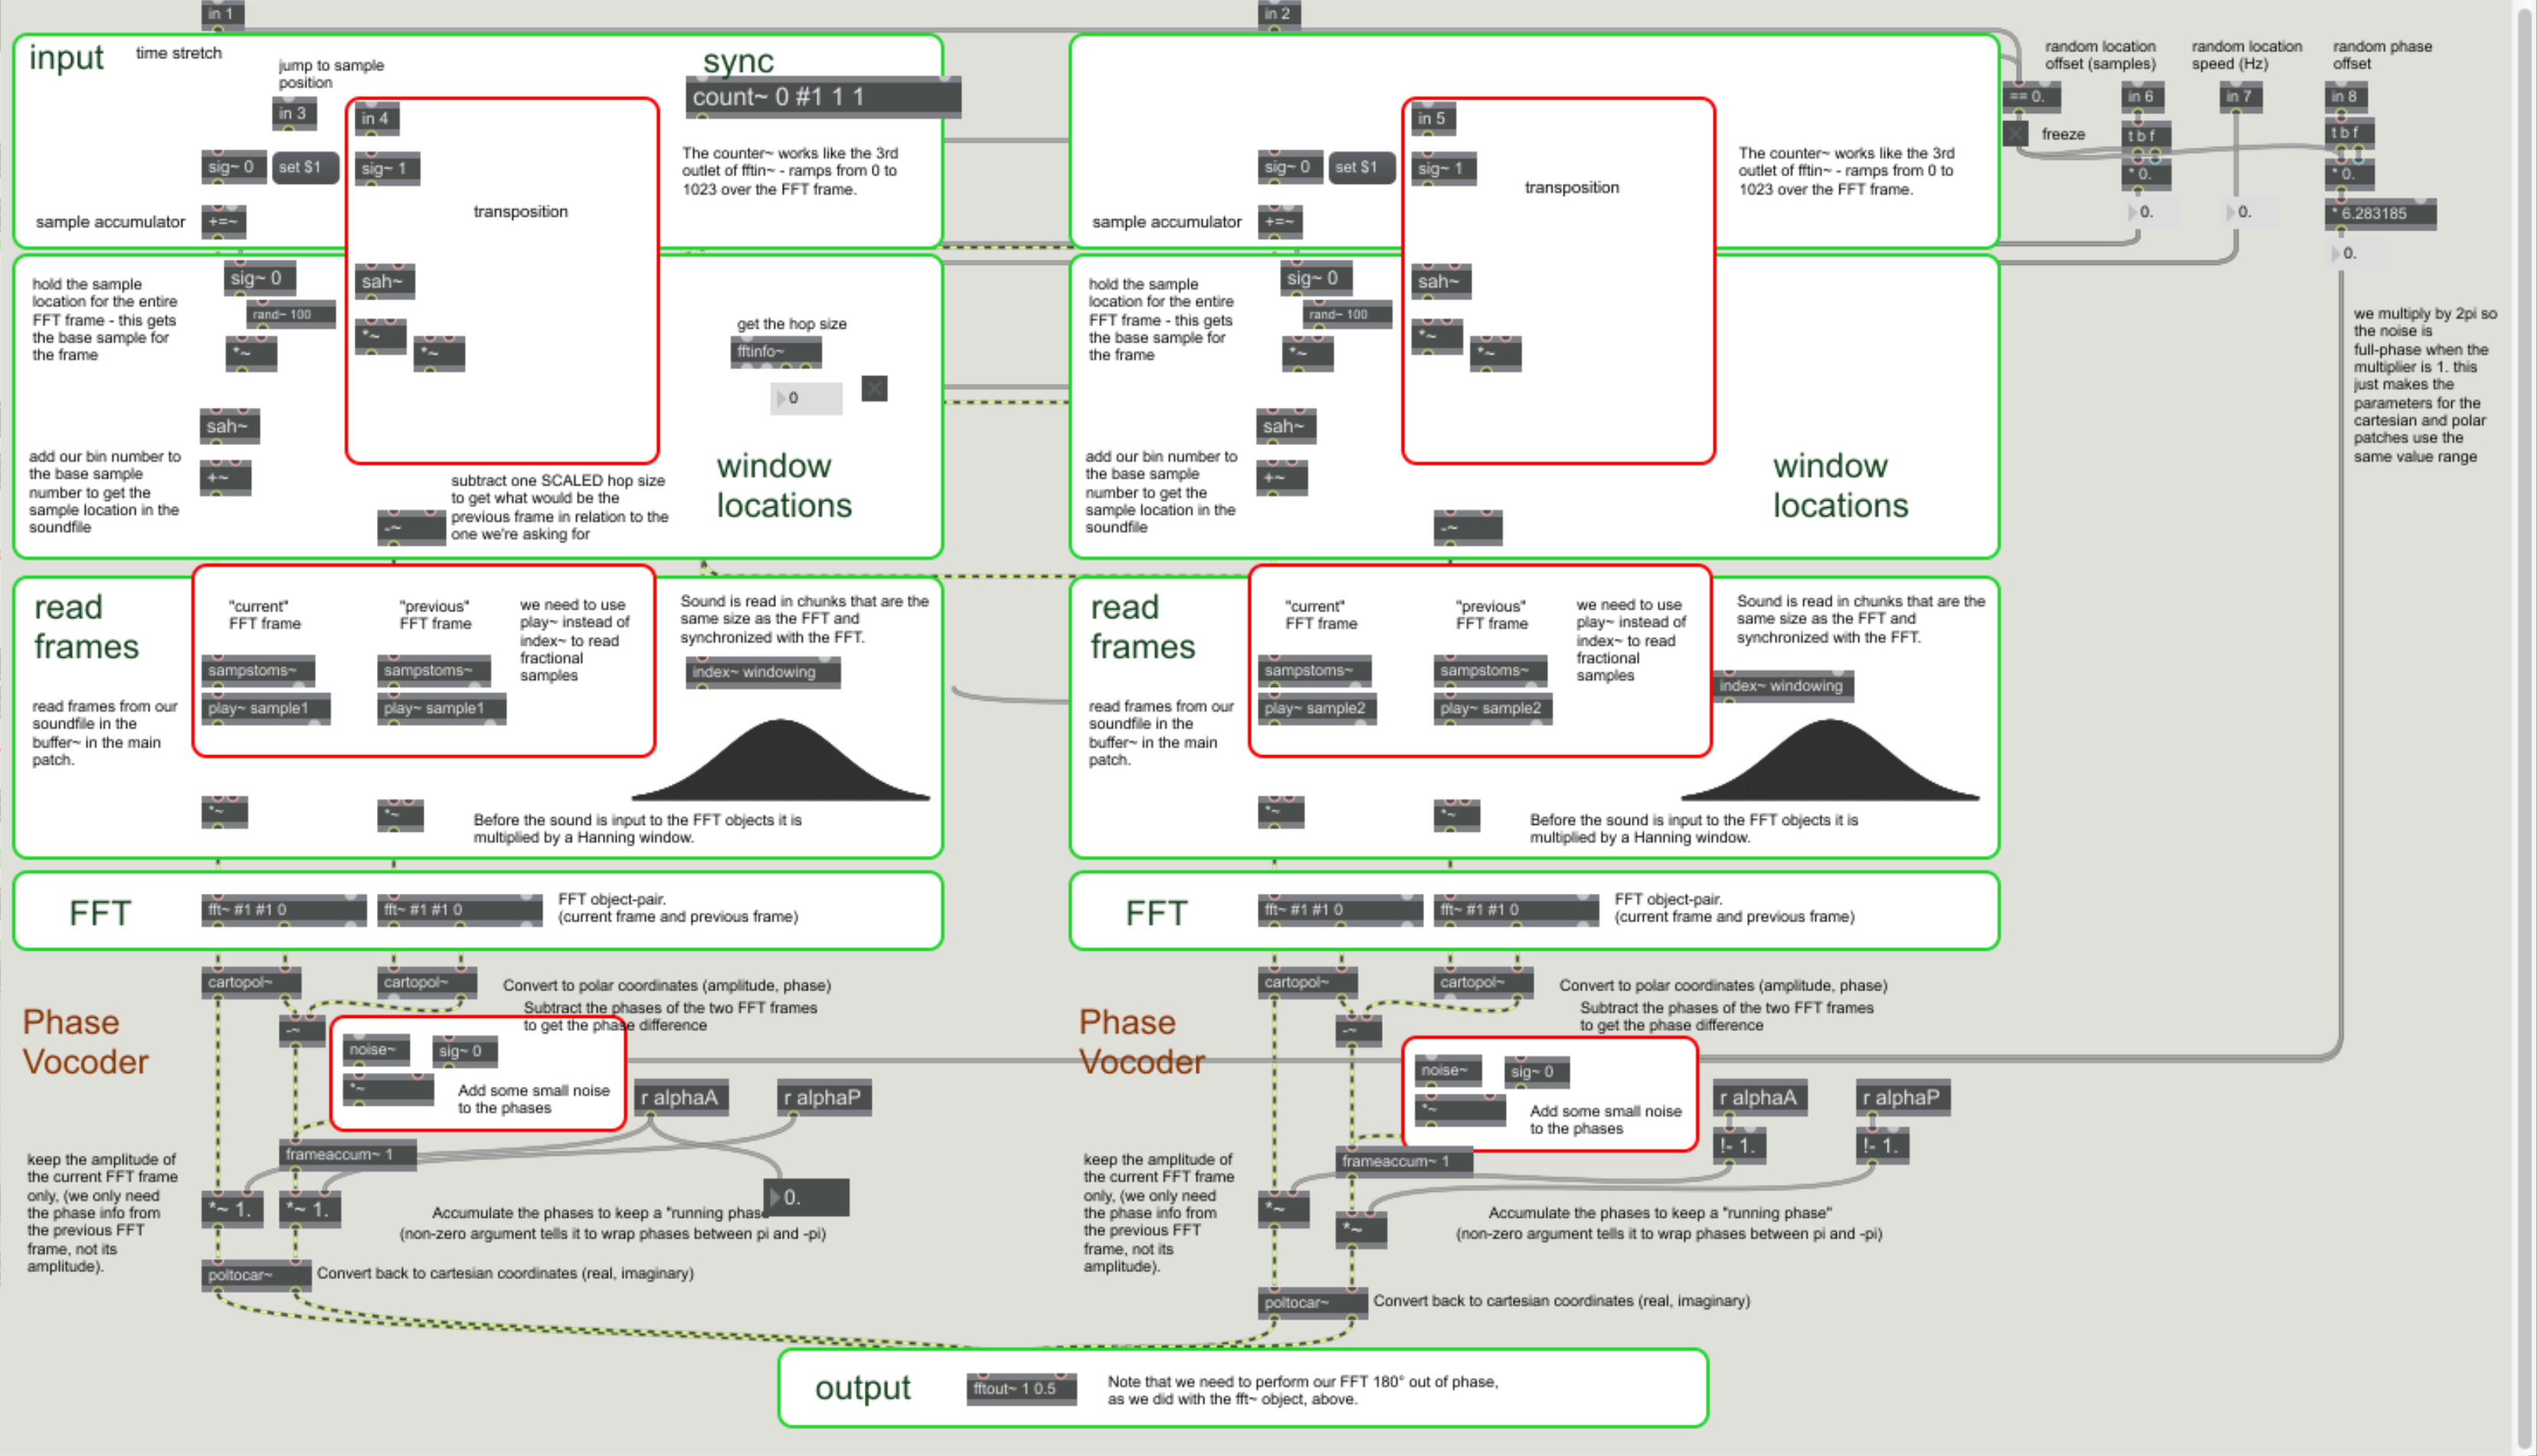
\includegraphics[width = \textwidth]{Graphs/SuperPhaseVoc.png}
        \caption{Super Phase Vocoder II}
        \label{SuperPhaseVoc}
    \end{figure}

\subsection{Phase interference}
    In this MaxMSP patch we investigate a modification to the polar coordinates after the analysis stade. We simply add a phasor oscillator after the FFT and apply it to each magnitude and corrected phase of the window. This way the identity of the signal is not altered but an oscilating frequency interferes with every index of the FFT window. The patch can be viewed in the figure . The formula of this modification is presented bellow by the synthesis equation.

    \begin{equation}
      y(n, k) = \sum_{k=1}^K (A[n]+phi(n)) \; e^{j (\theta_k(n) +\phi(n)}
    \end{equation}
    
    Where y(n, k) is the windowed signal after the analysis. K is the number of sinisuoids, $A[n]$ is the instantaneous magnitude, $\theta$ is the instantaneous phase and $\phi(n)$ is the instantaneous phasor given by the formula :

    \begin{equation*}
        \phi(n) = n - floor(n)
    \end{equation*}

    We can see that, the underlying model of the FFT is used to represent this modification. Other models could perfectly describe this effect but in this version it is more direct.

\subsection{Modulation au bruit}
    In this Phase Vocoder we investigate a noise modulation on the frequency component. We add the noise component and we tried some different noise generators such as $rand\thicksim$, pink-noise, white-noise and simultaneously we controlled the amplitude factor of this noise component. The sub-patch for noise selection can be seen in figure \ref{Noise_Select}.

    \begin{figure}
        \centering
        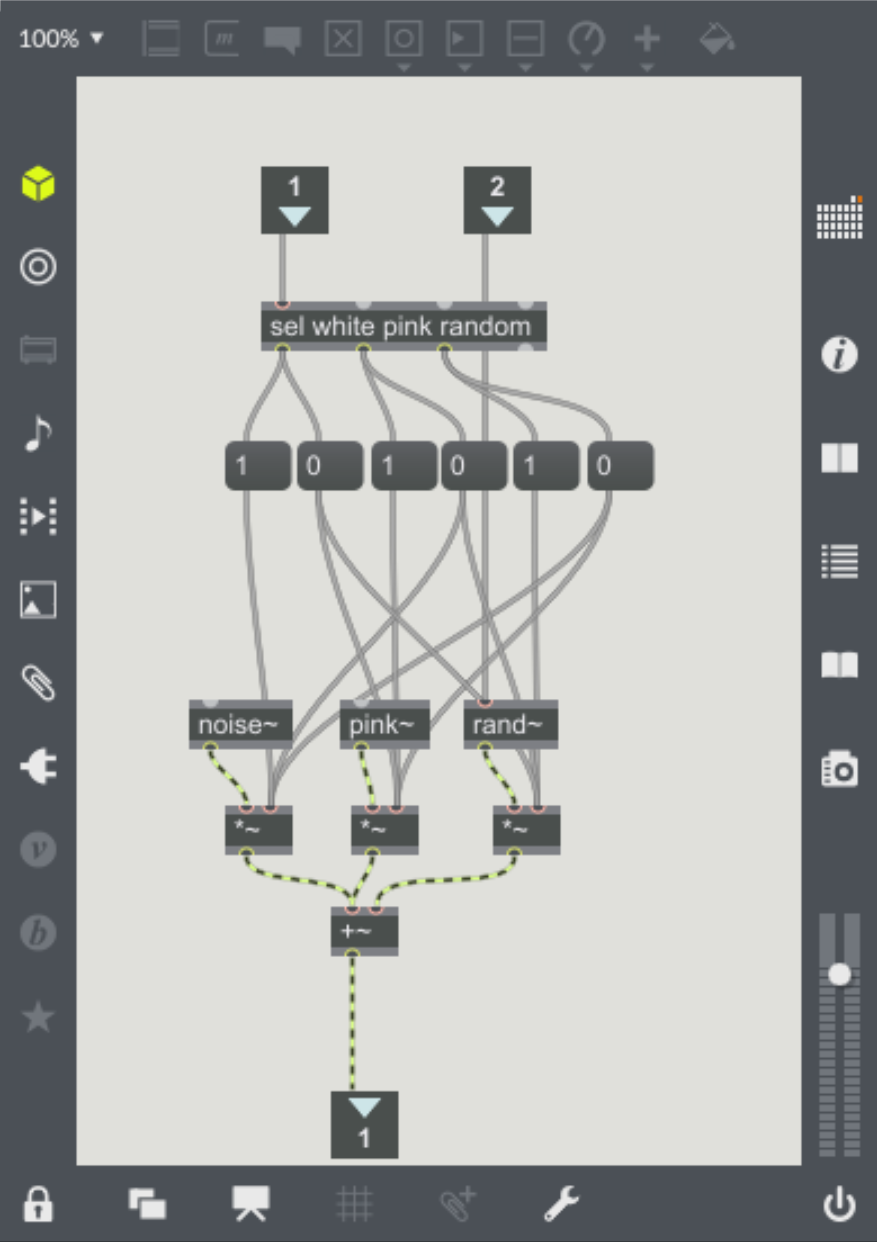
\includegraphics[width = \textwidth ]{Graphs/Noise_Select.png}
        \caption{Selection du bruit}
        \label{Noise_Select}
    \end{figure}

\subsection{Filtre aletoire sur la position du buffer$\thicksim$}

    In this patch we modulate the position of the buffer through a random signal generator that passes it's values to the reader of the file position. The random generator is created by the object $random\thicksim$ with a filter modulating the frequency of the random value generation The values that passes into the reader of the $play\thicksim$ object is modulated by a sample holder that takes as inputs the output of a counter and the random generated value. The sample holder is created manually by a greater than object and a gate. In this manner we hold and release abstractly values within the FFT window creating a hybrid of pitch and playback modulation. The modulation can be found in figure \ref{random_sampling}.

    \begin{figure}
        \centering
        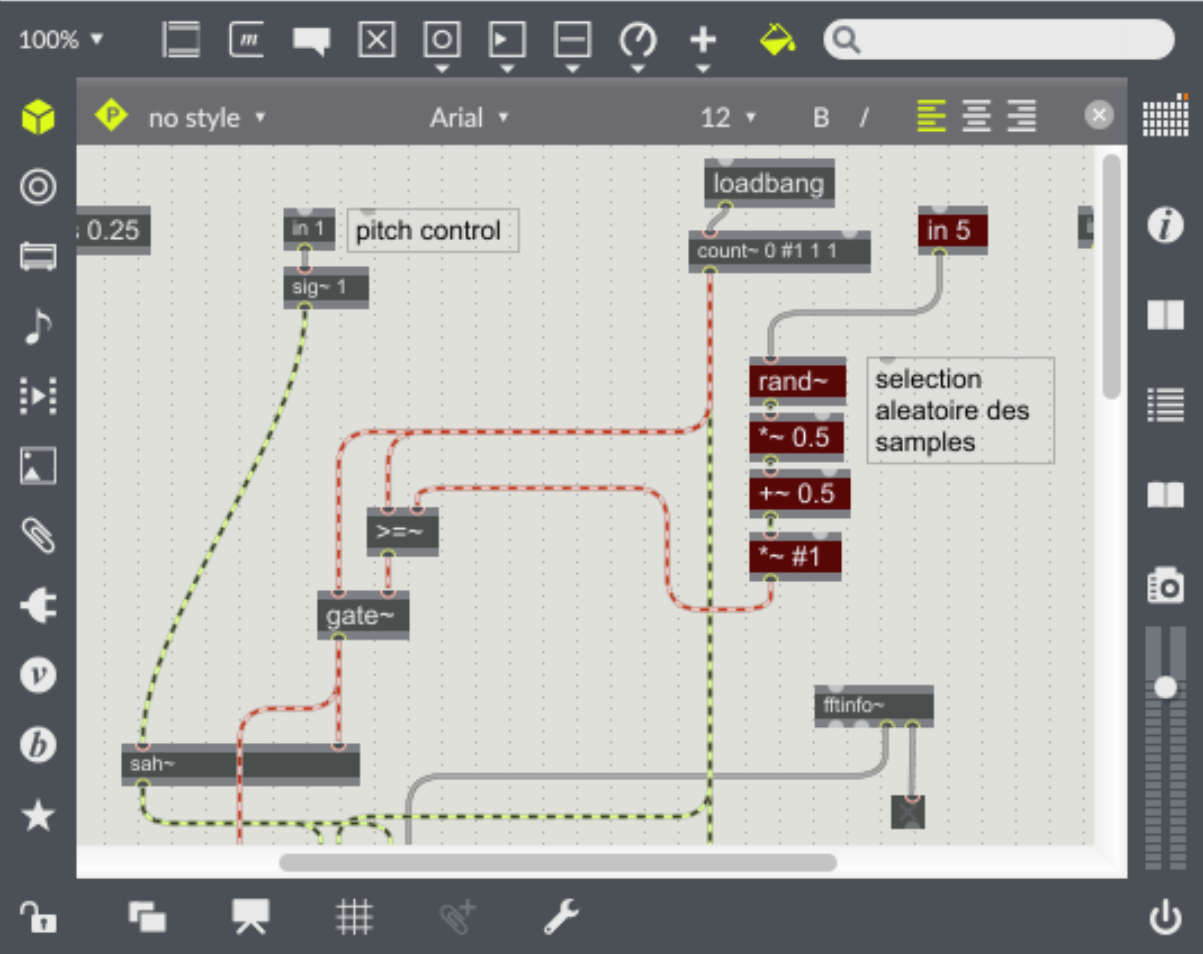
\includegraphics[width = \textwidth ]{Graphs/random_sampling.png}
        \caption{Filtre aletoire}
        \label{random_sampling}
    \end{figure}
    

\section{Morphing visuel}

En avançant sur le morphing visuel, nous avons implémenté le patch suivant avec l’aide du Jitter, pour une interpolation linéaire entre deux dessins.

    \begin{figure}
        \centering
        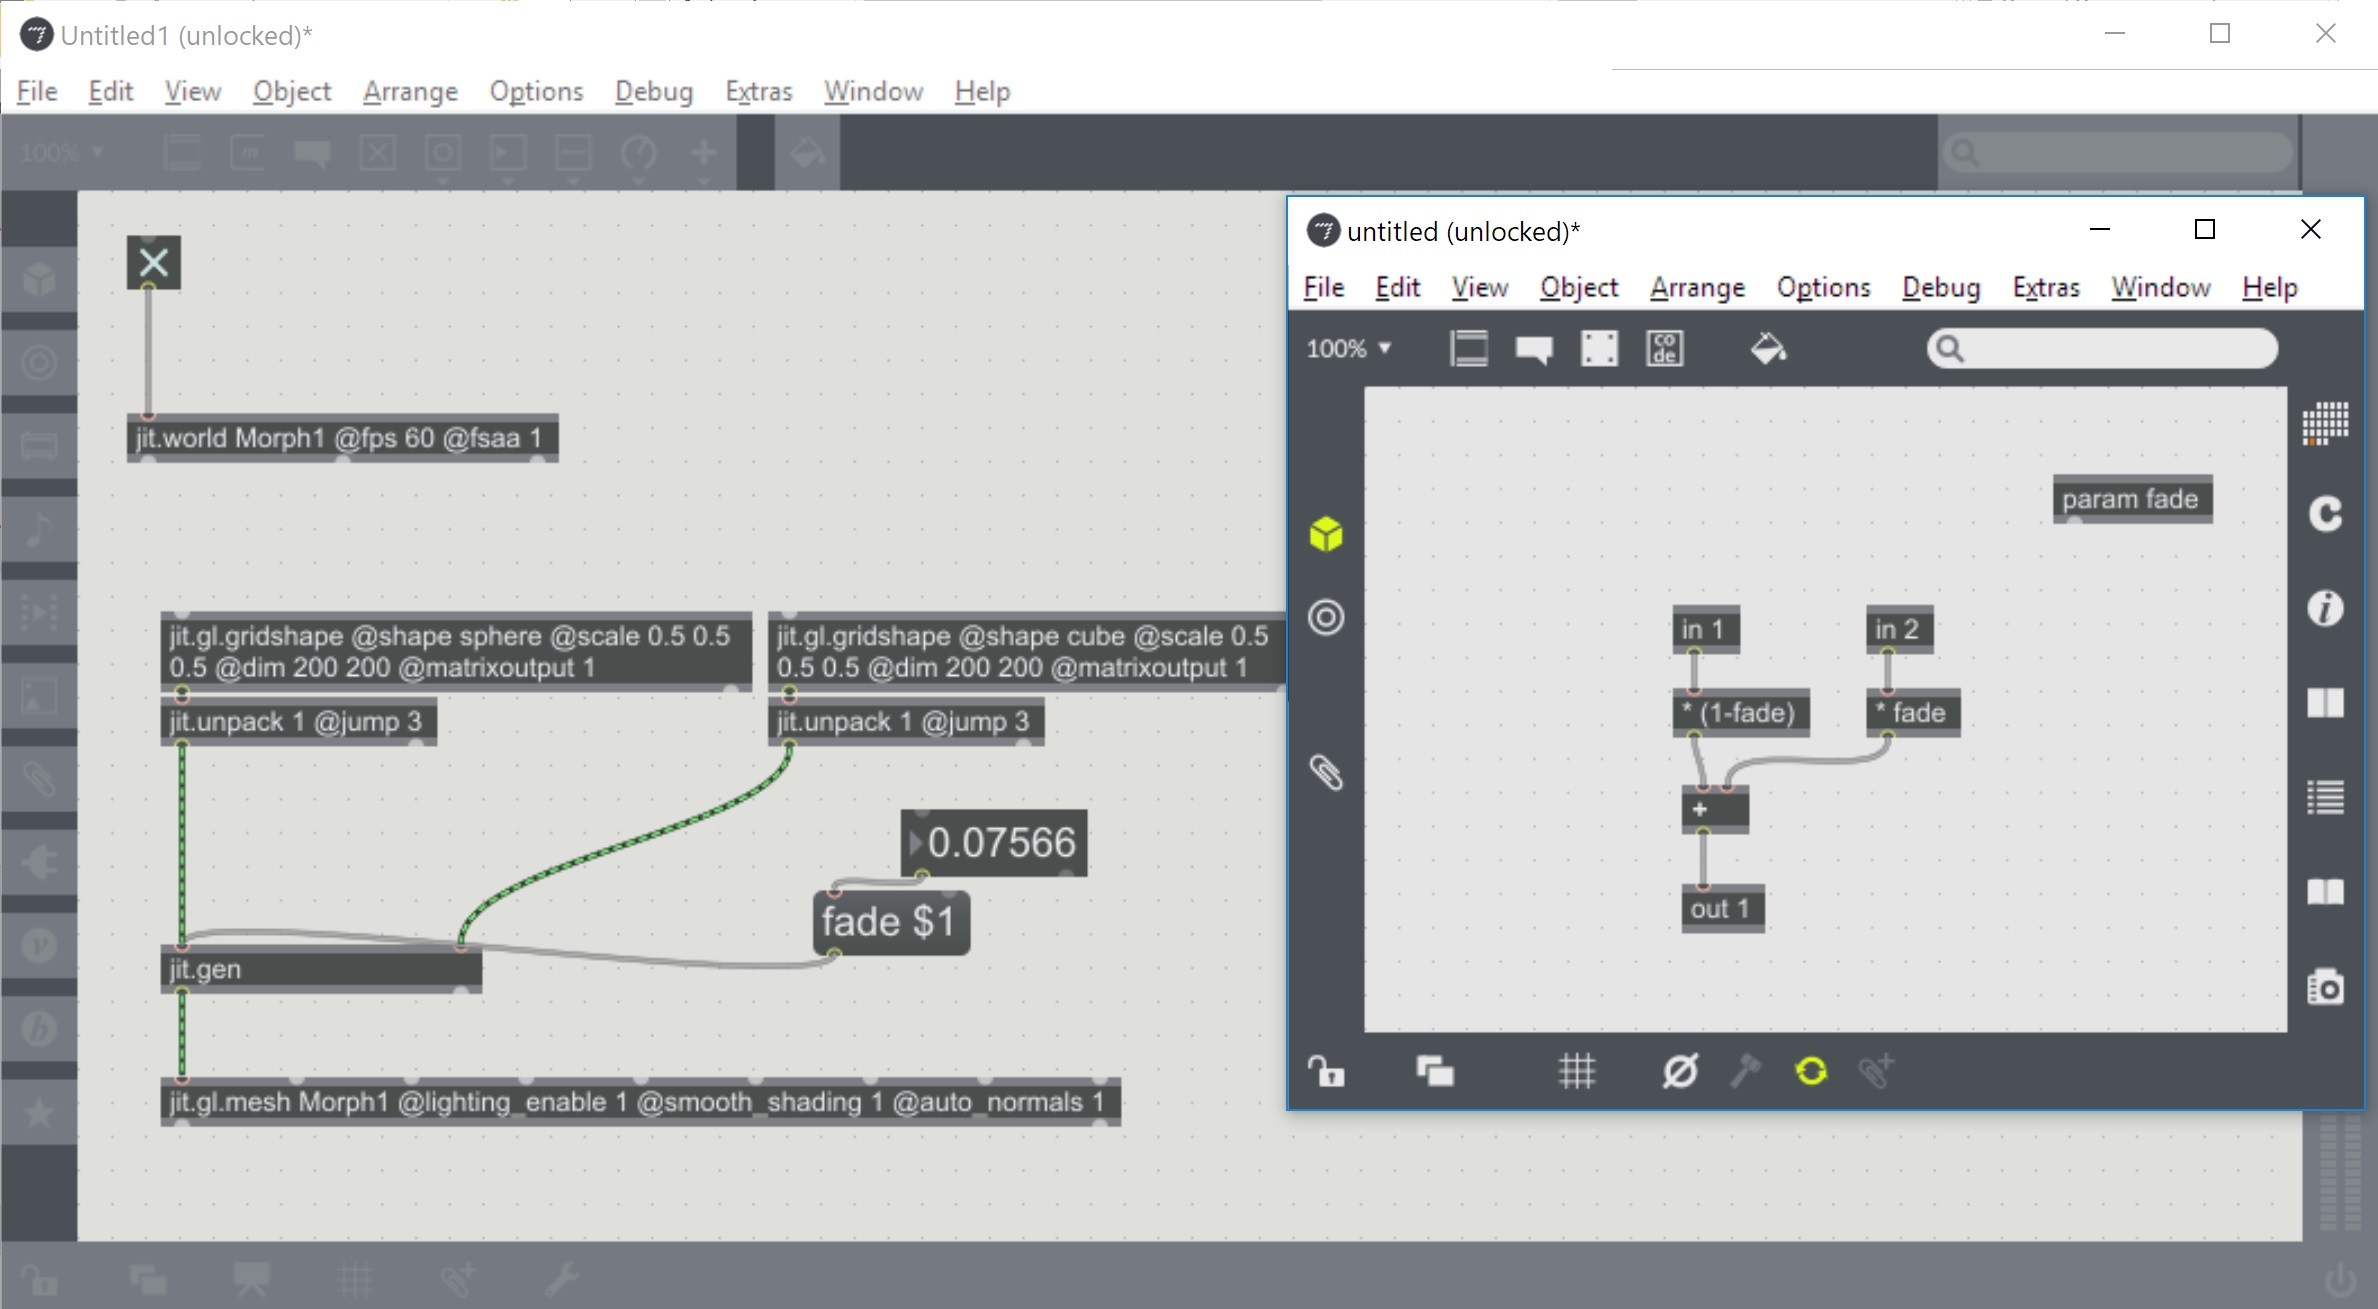
\includegraphics[width = \textwidth ]{Graphs/Morphing_patch.png}
        \caption{Visual Morphing}
        \label{VisualMorph}
    \end{figure}


En répétant la formule de base de morphing $M(\alpha) = \alpha\widehat {S_1} + [1 -\alpha]\widehat {S_2} $ une patch sur le morphing en 3D était implémenté avec l'aide de l'objet jit.gen (figure \ref{VisualMorph}).

Donc, fondamentalement, un morphing visuel est facile à faire avec les fonctions 3D primordiaux de Jitter telles que jit.gl.gridshape et jit.gen pour une personnalisation de la procédure de morphing. L'objet jit.gl.mesh est utilisé pour combiner le résultat du morphing alors que l'objet gen est contrôlé par un facteur de fondu.

À l'intérieur de gen, une procédure assez simple se produit. Les données multidimensionnelles provenant des matrices de localisation sont utilisées séparément pour chaque forme et leur amplitude est multipliée par le facteur $\alpha$ comme dans le morphing audio.

Bien entendu, nous pourrions également implémenter le script expondential.js pour une courbe de morphing différente sur le visuel.

Dans le patch suivant nous sommes allés un etape plus loin en separent tout composant d'un modèle tri-dimensionel dans jitter. Nous distinguons les valeurs des matrices, des normals et de la texture. Nous avons ajoutés egalement une interpolation du couleur. Le patch est en disposition en figure \ref{VisualMorph2}.

    \begin{figure}
        \centering
        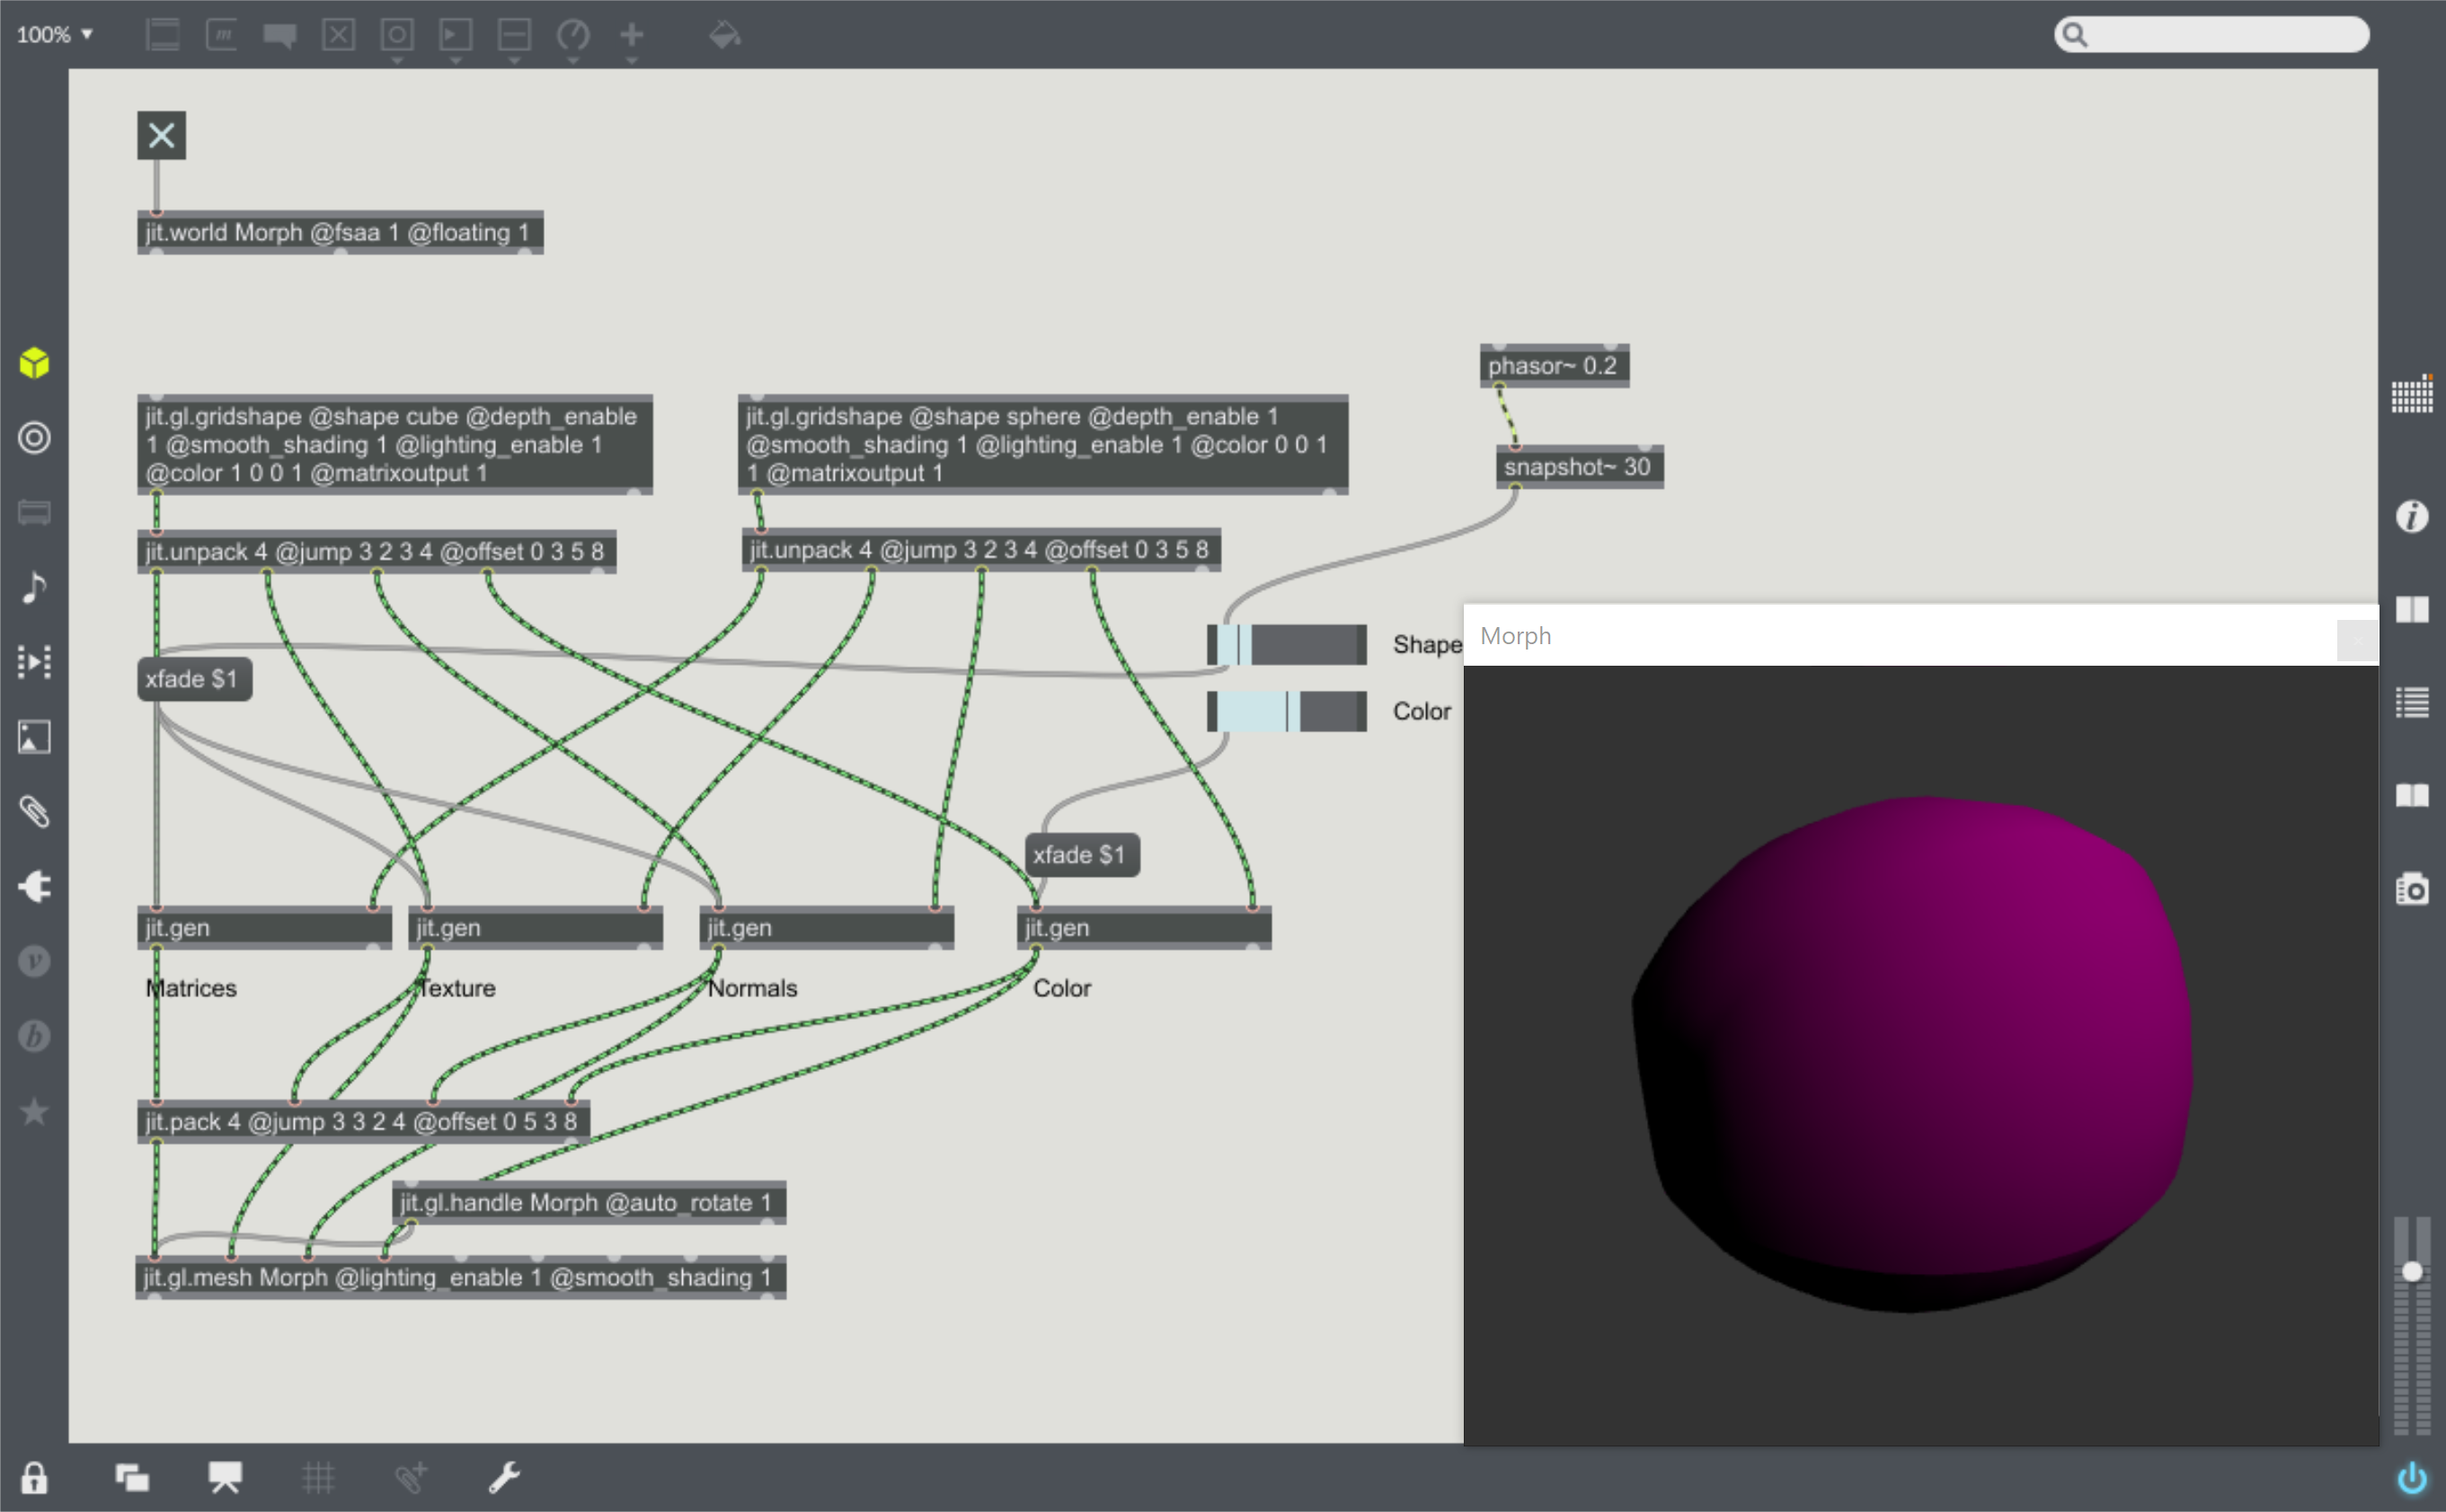
\includegraphics[width = \textwidth ]{Graphs/ShapeMorphing1.png}
        \caption{Visual Morphing $2{ème}$ version}
        \label{VisualMorph2}
    \end{figure} 

\begin{figure}
\begin{subfigure}{.5\textwidth}
  \centering
  % include first image
  \includegraphics[width=.8\linewidth]{log_demo1.png}  
  \caption{Put your sub-caption here}
  \label{fig:sub-first}
\end{subfigure}
\begin{subfigure}{.5\textwidth}
  \centering
  % include second image
  \includegraphics[width=.8\linewidth]{log_demo2.png}  
  \caption{Put your sub-caption here}
  \label{fig:sub-second}
\end{subfigure}

\newline

\begin{subfigure}{.5\textwidth}
  \centering
  % include third image
  \includegraphics[width=.8\linewidth]{log_demo1.png}  
  \caption{Put your sub-caption here}
  \label{fig:sub-third}
\end{subfigure}
\begin{subfigure}{.5\textwidth}
  \centering
  % include fourth image
  \includegraphics[width=.8\linewidth]{log_demo2.png}  
  \caption{Put your sub-caption here}
  \label{fig:sub-fourth}
\end{subfigure}
\caption{Put your caption here}
\label{fig:fig}
\end{figure}

\subsection{Visualization du spectre}
    
    In this patch a lot of Jitter work was implemented along with a Phase Vocoder. This code allows to visualize the spectral information of a sound as a packet of two dimensional lines mimicking the harmonics found from a Fourier Analysis.

    This patch used in unison with a phase Vocoder for morphing or even simple pitch shifting one can visualize the change of the spectrum in a real-time rendering environment. In this code we use an additional jitter library to produce multiple jitter objects rendered in virtual three dimensional space. The objective of this dissertation is not image oriented thus we won't unveil a lot of processing information.

    Here we will attribute briefly the most iconic jitter objects used in this patch. The \textit{jit.world} object creates a new window and a three dimensional virtual rendering space that also could contain physics, planes, three dimensional objects, control the camera position, the background color and a lot more. The \textit{jit.gridshape} renders a three dimensional object into a window. The \textit{jit.mo} library replicates copies of jitter objects in a smooth manner. And the \textit{jit.catch} takes a signal and translates it into a jitter matrix for potential visualization.

    For transforming the spectral information into three dimensional data we use of course an FFT transform and a buffer that reads the polar components of the FFT (magnitude and phase) by a $peek\thicksim$ object sends them into a buffer. An object $lookup\thicksim$ recuperates the contents of the buffer and inputs them into the \textit{jit.catch} object.

    We can regulate the dimension of the \textit{jit.mo} to output more harmonics. The output sound of the vocoder is sent to this harmonic visualization patch to grasp the result in a 3D space.

